\documentclass[]{article}
\usepackage{lmodern}
\usepackage{amssymb,amsmath}
\usepackage{ifxetex,ifluatex}
\usepackage{fixltx2e} % provides \textsubscript
\ifnum 0\ifxetex 1\fi\ifluatex 1\fi=0 % if pdftex
  \usepackage[T1]{fontenc}
  \usepackage[utf8]{inputenc}
\else % if luatex or xelatex
  \ifxetex
    \usepackage{mathspec}
  \else
    \usepackage{fontspec}
  \fi
  \defaultfontfeatures{Ligatures=TeX,Scale=MatchLowercase}
\fi
% use upquote if available, for straight quotes in verbatim environments
\IfFileExists{upquote.sty}{\usepackage{upquote}}{}
% use microtype if available
\IfFileExists{microtype.sty}{%
\usepackage{microtype}
\UseMicrotypeSet[protrusion]{basicmath} % disable protrusion for tt fonts
}{}
\usepackage[margin=2.54cm]{geometry}
\usepackage{hyperref}
\hypersetup{unicode=true,
            pdftitle={Assignment 6: Generalized Linear Models},
            pdfauthor={Connie Xiong},
            pdfborder={0 0 0},
            breaklinks=true}
\urlstyle{same}  % don't use monospace font for urls
\usepackage{color}
\usepackage{fancyvrb}
\newcommand{\VerbBar}{|}
\newcommand{\VERB}{\Verb[commandchars=\\\{\}]}
\DefineVerbatimEnvironment{Highlighting}{Verbatim}{commandchars=\\\{\}}
% Add ',fontsize=\small' for more characters per line
\usepackage{framed}
\definecolor{shadecolor}{RGB}{248,248,248}
\newenvironment{Shaded}{\begin{snugshade}}{\end{snugshade}}
\newcommand{\KeywordTok}[1]{\textcolor[rgb]{0.13,0.29,0.53}{\textbf{#1}}}
\newcommand{\DataTypeTok}[1]{\textcolor[rgb]{0.13,0.29,0.53}{#1}}
\newcommand{\DecValTok}[1]{\textcolor[rgb]{0.00,0.00,0.81}{#1}}
\newcommand{\BaseNTok}[1]{\textcolor[rgb]{0.00,0.00,0.81}{#1}}
\newcommand{\FloatTok}[1]{\textcolor[rgb]{0.00,0.00,0.81}{#1}}
\newcommand{\ConstantTok}[1]{\textcolor[rgb]{0.00,0.00,0.00}{#1}}
\newcommand{\CharTok}[1]{\textcolor[rgb]{0.31,0.60,0.02}{#1}}
\newcommand{\SpecialCharTok}[1]{\textcolor[rgb]{0.00,0.00,0.00}{#1}}
\newcommand{\StringTok}[1]{\textcolor[rgb]{0.31,0.60,0.02}{#1}}
\newcommand{\VerbatimStringTok}[1]{\textcolor[rgb]{0.31,0.60,0.02}{#1}}
\newcommand{\SpecialStringTok}[1]{\textcolor[rgb]{0.31,0.60,0.02}{#1}}
\newcommand{\ImportTok}[1]{#1}
\newcommand{\CommentTok}[1]{\textcolor[rgb]{0.56,0.35,0.01}{\textit{#1}}}
\newcommand{\DocumentationTok}[1]{\textcolor[rgb]{0.56,0.35,0.01}{\textbf{\textit{#1}}}}
\newcommand{\AnnotationTok}[1]{\textcolor[rgb]{0.56,0.35,0.01}{\textbf{\textit{#1}}}}
\newcommand{\CommentVarTok}[1]{\textcolor[rgb]{0.56,0.35,0.01}{\textbf{\textit{#1}}}}
\newcommand{\OtherTok}[1]{\textcolor[rgb]{0.56,0.35,0.01}{#1}}
\newcommand{\FunctionTok}[1]{\textcolor[rgb]{0.00,0.00,0.00}{#1}}
\newcommand{\VariableTok}[1]{\textcolor[rgb]{0.00,0.00,0.00}{#1}}
\newcommand{\ControlFlowTok}[1]{\textcolor[rgb]{0.13,0.29,0.53}{\textbf{#1}}}
\newcommand{\OperatorTok}[1]{\textcolor[rgb]{0.81,0.36,0.00}{\textbf{#1}}}
\newcommand{\BuiltInTok}[1]{#1}
\newcommand{\ExtensionTok}[1]{#1}
\newcommand{\PreprocessorTok}[1]{\textcolor[rgb]{0.56,0.35,0.01}{\textit{#1}}}
\newcommand{\AttributeTok}[1]{\textcolor[rgb]{0.77,0.63,0.00}{#1}}
\newcommand{\RegionMarkerTok}[1]{#1}
\newcommand{\InformationTok}[1]{\textcolor[rgb]{0.56,0.35,0.01}{\textbf{\textit{#1}}}}
\newcommand{\WarningTok}[1]{\textcolor[rgb]{0.56,0.35,0.01}{\textbf{\textit{#1}}}}
\newcommand{\AlertTok}[1]{\textcolor[rgb]{0.94,0.16,0.16}{#1}}
\newcommand{\ErrorTok}[1]{\textcolor[rgb]{0.64,0.00,0.00}{\textbf{#1}}}
\newcommand{\NormalTok}[1]{#1}
\usepackage{graphicx,grffile}
\makeatletter
\def\maxwidth{\ifdim\Gin@nat@width>\linewidth\linewidth\else\Gin@nat@width\fi}
\def\maxheight{\ifdim\Gin@nat@height>\textheight\textheight\else\Gin@nat@height\fi}
\makeatother
% Scale images if necessary, so that they will not overflow the page
% margins by default, and it is still possible to overwrite the defaults
% using explicit options in \includegraphics[width, height, ...]{}
\setkeys{Gin}{width=\maxwidth,height=\maxheight,keepaspectratio}
\IfFileExists{parskip.sty}{%
\usepackage{parskip}
}{% else
\setlength{\parindent}{0pt}
\setlength{\parskip}{6pt plus 2pt minus 1pt}
}
\setlength{\emergencystretch}{3em}  % prevent overfull lines
\providecommand{\tightlist}{%
  \setlength{\itemsep}{0pt}\setlength{\parskip}{0pt}}
\setcounter{secnumdepth}{0}
% Redefines (sub)paragraphs to behave more like sections
\ifx\paragraph\undefined\else
\let\oldparagraph\paragraph
\renewcommand{\paragraph}[1]{\oldparagraph{#1}\mbox{}}
\fi
\ifx\subparagraph\undefined\else
\let\oldsubparagraph\subparagraph
\renewcommand{\subparagraph}[1]{\oldsubparagraph{#1}\mbox{}}
\fi

%%% Use protect on footnotes to avoid problems with footnotes in titles
\let\rmarkdownfootnote\footnote%
\def\footnote{\protect\rmarkdownfootnote}

%%% Change title format to be more compact
\usepackage{titling}

% Create subtitle command for use in maketitle
\newcommand{\subtitle}[1]{
  \posttitle{
    \begin{center}\large#1\end{center}
    }
}

\setlength{\droptitle}{-2em}

  \title{Assignment 6: Generalized Linear Models}
    \pretitle{\vspace{\droptitle}\centering\huge}
  \posttitle{\par}
    \author{Connie Xiong}
    \preauthor{\centering\large\emph}
  \postauthor{\par}
    \date{}
    \predate{}\postdate{}
  

\begin{document}
\maketitle

\subsection{OVERVIEW}\label{overview}

This exercise accompanies the lessons in Environmental Data Analytics
(ENV872L) on generalized linear models.

\subsection{Directions}\label{directions}

\begin{enumerate}
\def\labelenumi{\arabic{enumi}.}
\tightlist
\item
  Change ``Student Name'' on line 3 (above) with your name.
\item
  Use the lesson as a guide. It contains code that can be modified to
  complete the assignment.
\item
  Work through the steps, \textbf{creating code and output} that fulfill
  each instruction.
\item
  Be sure to \textbf{answer the questions} in this assignment document.
  Space for your answers is provided in this document and is indicated
  by the ``\textgreater{}'' character. If you need a second paragraph be
  sure to start the first line with ``\textgreater{}''. You should
  notice that the answer is highlighted in green by RStudio.
\item
  When you have completed the assignment, \textbf{Knit} the text and
  code into a single PDF file. You will need to have the correct
  software installed to do this (see Software Installation Guide) Press
  the \texttt{Knit} button in the RStudio scripting panel. This will
  save the PDF output in your Assignments folder.
\item
  After Knitting, please submit the completed exercise (PDF file) to the
  dropbox in Sakai. Please add your last name into the file name (e.g.,
  ``Salk\_A06\_GLMs.pdf'') prior to submission.
\end{enumerate}

The completed exercise is due on Tuesday, 26 February, 2019 before class
begins.

\subsection{Set up your session}\label{set-up-your-session}

\begin{enumerate}
\def\labelenumi{\arabic{enumi}.}
\item
  Set up your session. Upload the EPA Ecotox dataset for Neonicotinoids
  and the NTL-LTER raw data file for chemistry/physics.
\item
  Build a ggplot theme and set it as your default theme.
\end{enumerate}

\begin{Shaded}
\begin{Highlighting}[]
\CommentTok{#1}
\KeywordTok{getwd}\NormalTok{()}
\end{Highlighting}
\end{Shaded}

\begin{verbatim}
## [1] "C:/Users/Wanch/Desktop/ENVI 872 data/Environmental_Data_Analytics"
\end{verbatim}

\begin{Shaded}
\begin{Highlighting}[]
\KeywordTok{library}\NormalTok{(tidyverse)}
\end{Highlighting}
\end{Shaded}

\begin{verbatim}
## -- Attaching packages ---------------------------------------------- tidyverse 1.2.1 --
\end{verbatim}

\begin{verbatim}
## v ggplot2 3.1.0     v purrr   0.2.5
## v tibble  2.0.1     v dplyr   0.7.8
## v tidyr   0.8.2     v stringr 1.3.1
## v readr   1.3.1     v forcats 0.3.0
\end{verbatim}

\begin{verbatim}
## -- Conflicts ------------------------------------------------- tidyverse_conflicts() --
## x dplyr::filter() masks stats::filter()
## x dplyr::lag()    masks stats::lag()
\end{verbatim}

\begin{Shaded}
\begin{Highlighting}[]
\NormalTok{ecotox <-}\StringTok{ }\KeywordTok{read.csv}\NormalTok{(}\StringTok{"./Data/Raw/ECOTOX_Neonicotinoids_Mortality_raw.csv"}\NormalTok{)}

\NormalTok{chem.phys <-}\StringTok{ }\KeywordTok{read.csv}\NormalTok{(}\StringTok{"./Data/Raw/NTL-LTER_Lake_ChemistryPhysics_Raw.csv"}\NormalTok{)}

\CommentTok{#2}
\NormalTok{mytheme <-}\StringTok{ }\KeywordTok{theme_grey}\NormalTok{() }\OperatorTok{+}
\StringTok{  }\KeywordTok{theme}\NormalTok{(}\DataTypeTok{axis.text =} \KeywordTok{element_text}\NormalTok{(}\DataTypeTok{color =} \StringTok{"black"}\NormalTok{), }
        \DataTypeTok{legend.position =} \StringTok{"right"}\NormalTok{)}
\KeywordTok{theme_set}\NormalTok{(mytheme)}
\end{Highlighting}
\end{Shaded}

\subsection{Neonicotinoids test}\label{neonicotinoids-test}

Research question: Were studies on various neonicotinoid chemicals
conducted in different years?

\begin{enumerate}
\def\labelenumi{\arabic{enumi}.}
\setcounter{enumi}{2}
\item
  Generate a line of code to determine how many different chemicals are
  listed in the Chemical.Name column.
\item
  Are the publication years associated with each chemical
  well-approximated by a normal distribution? Run the appropriate test
  and also generate a frequency polygon to illustrate the distribution
  of counts for each year, divided by chemical name. Bonus points if you
  can generate the results of your test from a pipe function. No need to
  make this graph pretty.
\item
  Is there equal variance among the publication years for each chemical?
  Hint: var.test is not the correct function.
\end{enumerate}

\begin{Shaded}
\begin{Highlighting}[]
\CommentTok{#3 Check how many chemicals are in the dataset}
\KeywordTok{str}\NormalTok{(ecotox}\OperatorTok{$}\NormalTok{Chemical.Name)}
\end{Highlighting}
\end{Shaded}

\begin{verbatim}
##  Factor w/ 9 levels "Acetamiprid",..: 4 8 4 4 8 8 8 8 4 4 ...
\end{verbatim}

\begin{Shaded}
\begin{Highlighting}[]
\CommentTok{#4 Determine whether publication years associated with each chemical is well-approximated by a normal distribution; generate a frequency polygon to see the distribution of counts for each year}
\KeywordTok{shapiro.test}\NormalTok{(ecotox}\OperatorTok{$}\NormalTok{Pub..Year[ecotox}\OperatorTok{$}\NormalTok{Chemical.Name }\OperatorTok{==}\StringTok{ "Acetamiprid"}\NormalTok{])}
\end{Highlighting}
\end{Shaded}

\begin{verbatim}
## 
##  Shapiro-Wilk normality test
## 
## data:  ecotox$Pub..Year[ecotox$Chemical.Name == "Acetamiprid"]
## W = 0.90191, p-value = 5.706e-08
\end{verbatim}

\begin{Shaded}
\begin{Highlighting}[]
\KeywordTok{shapiro.test}\NormalTok{(ecotox}\OperatorTok{$}\NormalTok{Pub..Year[ecotox}\OperatorTok{$}\NormalTok{Chemical.Name }\OperatorTok{==}\StringTok{ "Clothianidin"}\NormalTok{])}
\end{Highlighting}
\end{Shaded}

\begin{verbatim}
## 
##  Shapiro-Wilk normality test
## 
## data:  ecotox$Pub..Year[ecotox$Chemical.Name == "Clothianidin"]
## W = 0.69577, p-value = 4.287e-11
\end{verbatim}

\begin{Shaded}
\begin{Highlighting}[]
\KeywordTok{shapiro.test}\NormalTok{(ecotox}\OperatorTok{$}\NormalTok{Pub..Year[ecotox}\OperatorTok{$}\NormalTok{Chemical.Name }\OperatorTok{==}\StringTok{ "Dinotefuran"}\NormalTok{])}
\end{Highlighting}
\end{Shaded}

\begin{verbatim}
## 
##  Shapiro-Wilk normality test
## 
## data:  ecotox$Pub..Year[ecotox$Chemical.Name == "Dinotefuran"]
## W = 0.82848, p-value = 8.83e-07
\end{verbatim}

\begin{Shaded}
\begin{Highlighting}[]
\KeywordTok{shapiro.test}\NormalTok{(ecotox}\OperatorTok{$}\NormalTok{Pub..Year[ecotox}\OperatorTok{$}\NormalTok{Chemical.Name }\OperatorTok{==}\StringTok{ "Imidacloprid"}\NormalTok{])}
\end{Highlighting}
\end{Shaded}

\begin{verbatim}
## 
##  Shapiro-Wilk normality test
## 
## data:  ecotox$Pub..Year[ecotox$Chemical.Name == "Imidacloprid"]
## W = 0.88178, p-value < 2.2e-16
\end{verbatim}

\begin{Shaded}
\begin{Highlighting}[]
\KeywordTok{shapiro.test}\NormalTok{(ecotox}\OperatorTok{$}\NormalTok{Pub..Year[ecotox}\OperatorTok{$}\NormalTok{Chemical.Name }\OperatorTok{==}\StringTok{ "Imidaclothiz"}\NormalTok{])}
\end{Highlighting}
\end{Shaded}

\begin{verbatim}
## 
##  Shapiro-Wilk normality test
## 
## data:  ecotox$Pub..Year[ecotox$Chemical.Name == "Imidaclothiz"]
## W = 0.68429, p-value = 0.00093
\end{verbatim}

\begin{Shaded}
\begin{Highlighting}[]
\KeywordTok{shapiro.test}\NormalTok{(ecotox}\OperatorTok{$}\NormalTok{Pub..Year[ecotox}\OperatorTok{$}\NormalTok{Chemical.Name }\OperatorTok{==}\StringTok{ "Nitenpyram"}\NormalTok{])}
\end{Highlighting}
\end{Shaded}

\begin{verbatim}
## 
##  Shapiro-Wilk normality test
## 
## data:  ecotox$Pub..Year[ecotox$Chemical.Name == "Nitenpyram"]
## W = 0.79592, p-value = 0.0005686
\end{verbatim}

\begin{Shaded}
\begin{Highlighting}[]
\KeywordTok{shapiro.test}\NormalTok{(ecotox}\OperatorTok{$}\NormalTok{Pub..Year[ecotox}\OperatorTok{$}\NormalTok{Chemical.Name }\OperatorTok{==}\StringTok{ "Nithiazine"}\NormalTok{])}
\end{Highlighting}
\end{Shaded}

\begin{verbatim}
## 
##  Shapiro-Wilk normality test
## 
## data:  ecotox$Pub..Year[ecotox$Chemical.Name == "Nithiazine"]
## W = 0.75938, p-value = 0.0001235
\end{verbatim}

\begin{Shaded}
\begin{Highlighting}[]
\KeywordTok{shapiro.test}\NormalTok{(ecotox}\OperatorTok{$}\NormalTok{Pub..Year[ecotox}\OperatorTok{$}\NormalTok{Chemical.Name }\OperatorTok{==}\StringTok{ "Thiacloprid"}\NormalTok{])}
\end{Highlighting}
\end{Shaded}

\begin{verbatim}
## 
##  Shapiro-Wilk normality test
## 
## data:  ecotox$Pub..Year[ecotox$Chemical.Name == "Thiacloprid"]
## W = 0.7669, p-value = 1.118e-11
\end{verbatim}

\begin{Shaded}
\begin{Highlighting}[]
\KeywordTok{shapiro.test}\NormalTok{(ecotox}\OperatorTok{$}\NormalTok{Pub..Year[ecotox}\OperatorTok{$}\NormalTok{Chemical.Name }\OperatorTok{==}\StringTok{ "Thiamethoxam"}\NormalTok{])}
\end{Highlighting}
\end{Shaded}

\begin{verbatim}
## 
##  Shapiro-Wilk normality test
## 
## data:  ecotox$Pub..Year[ecotox$Chemical.Name == "Thiamethoxam"]
## W = 0.7071, p-value < 2.2e-16
\end{verbatim}

\begin{Shaded}
\begin{Highlighting}[]
\NormalTok{year.freq <-}\StringTok{ }\KeywordTok{ggplot}\NormalTok{(ecotox, }\KeywordTok{aes}\NormalTok{(}\DataTypeTok{x =}\NormalTok{ Pub..Year, }\DataTypeTok{color =}\NormalTok{ Chemical.Name)) }\OperatorTok{+}
\StringTok{         }\KeywordTok{geom_freqpoly}\NormalTok{(}\DataTypeTok{stat =} \StringTok{"count"}\NormalTok{)}
\KeywordTok{print}\NormalTok{(year.freq)}
\end{Highlighting}
\end{Shaded}

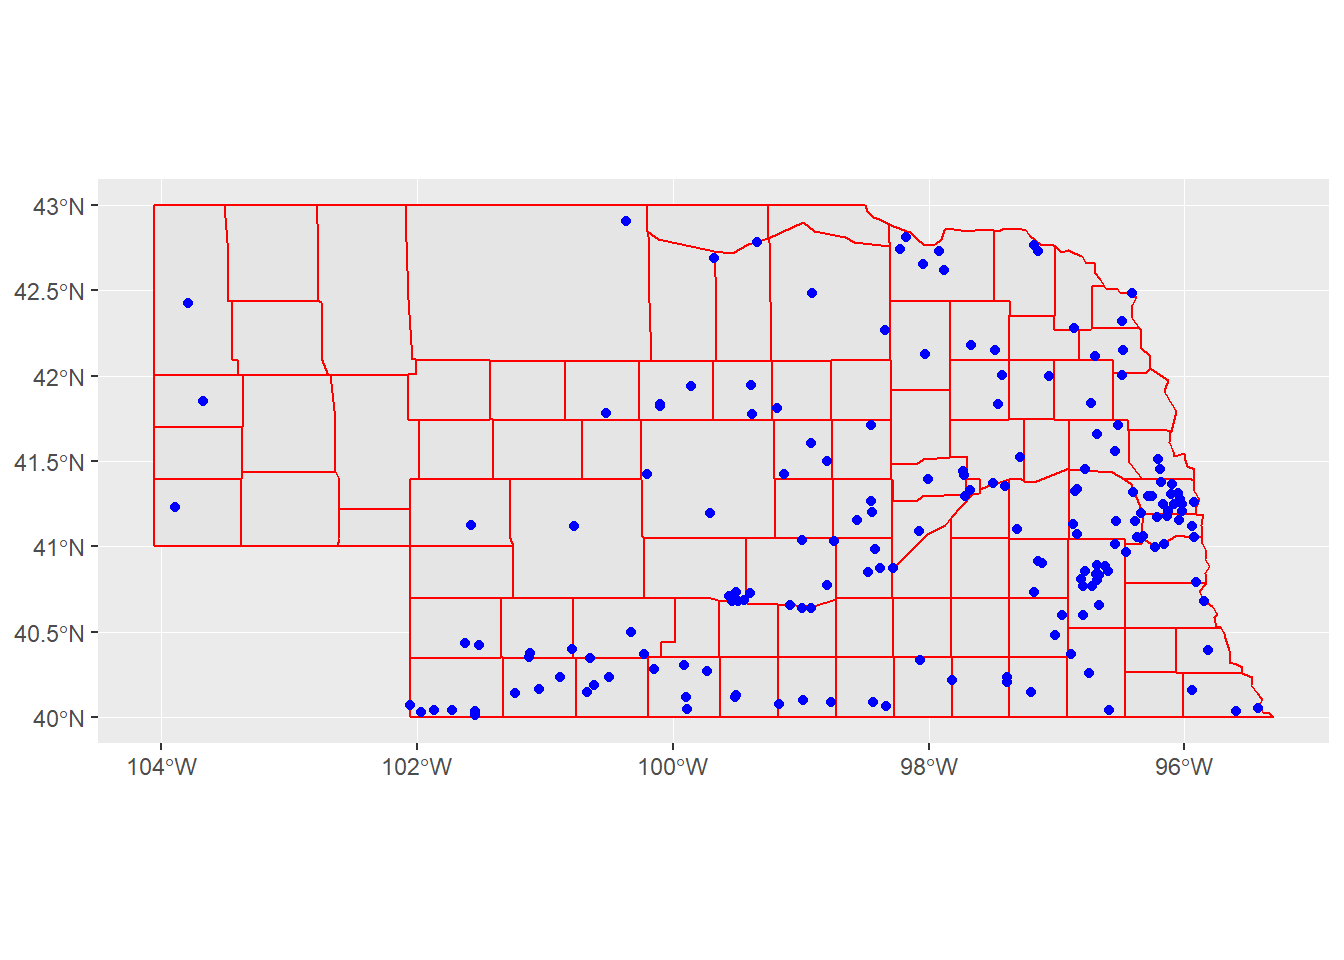
\includegraphics{A06_GLMs_files/figure-latex/unnamed-chunk-2-1.pdf}

\begin{Shaded}
\begin{Highlighting}[]
\CommentTok{#5 Check whether there is an equal variance among the publication years for each chemical}
\KeywordTok{bartlett.test}\NormalTok{(ecotox}\OperatorTok{$}\NormalTok{Pub..Year }\OperatorTok{~}\StringTok{ }\NormalTok{ecotox}\OperatorTok{$}\NormalTok{Chemical.Name)}
\end{Highlighting}
\end{Shaded}

\begin{verbatim}
## 
##  Bartlett test of homogeneity of variances
## 
## data:  ecotox$Pub..Year by ecotox$Chemical.Name
## Bartlett's K-squared = 139.59, df = 8, p-value < 2.2e-16
\end{verbatim}

\begin{enumerate}
\def\labelenumi{\arabic{enumi}.}
\setcounter{enumi}{5}
\tightlist
\item
  Based on your results, which test would you choose to run to answer
  your research question?
\end{enumerate}

\begin{quote}
ANSWER: I would choose ANOVA test to answer the research question.
\end{quote}

\begin{enumerate}
\def\labelenumi{\arabic{enumi}.}
\setcounter{enumi}{6}
\item
  Run this test below.
\item
  Generate a boxplot representing the range of publication years for
  each chemical. Adjust your graph to make it pretty.
\end{enumerate}

\begin{Shaded}
\begin{Highlighting}[]
\CommentTok{#7 Run an ANOVA test for the research question}
\NormalTok{pub.year.chemical.anova <-}\StringTok{ }\KeywordTok{lm}\NormalTok{(ecotox}\OperatorTok{$}\NormalTok{Pub..Year }\OperatorTok{~}\StringTok{ }\NormalTok{ecotox}\OperatorTok{$}\NormalTok{Chemical.Name)}
\KeywordTok{summary}\NormalTok{(pub.year.chemical.anova)}
\end{Highlighting}
\end{Shaded}

\begin{verbatim}
## 
## Call:
## lm(formula = ecotox$Pub..Year ~ ecotox$Chemical.Name)
## 
## Residuals:
##     Min      1Q  Median      3Q     Max 
## -18.366  -3.993   1.889   4.889  13.441 
## 
## Coefficients:
##                                   Estimate Std. Error  t value Pr(>|t|)
## (Intercept)                      2005.9926     0.6082 3298.222  < 2e-16
## ecotox$Chemical.NameClothianidin    2.0479     1.0246    1.999  0.04584
## ecotox$Chemical.NameDinotefuran    -3.4333     1.1057   -3.105  0.00194
## ecotox$Chemical.NameImidacloprid    3.1181     0.6651    4.689 3.05e-06
## ecotox$Chemical.NameImidaclothiz    6.4518     2.4412    2.643  0.00832
## ecotox$Chemical.NameNitenpyram      7.7216     1.6630    4.643 3.78e-06
## ecotox$Chemical.NameNithiazine    -17.6290     1.6299  -10.816  < 2e-16
## ecotox$Chemical.NameThiacloprid     1.6394     0.9190    1.784  0.07467
## ecotox$Chemical.NameThiamethoxam    4.3738     0.8261    5.295 1.40e-07
##                                     
## (Intercept)                      ***
## ecotox$Chemical.NameClothianidin *  
## ecotox$Chemical.NameDinotefuran  ** 
## ecotox$Chemical.NameImidacloprid ***
## ecotox$Chemical.NameImidaclothiz ** 
## ecotox$Chemical.NameNitenpyram   ***
## ecotox$Chemical.NameNithiazine   ***
## ecotox$Chemical.NameThiacloprid  .  
## ecotox$Chemical.NameThiamethoxam ***
## ---
## Signif. codes:  0 '***' 0.001 '**' 0.01 '*' 0.05 '.' 0.1 ' ' 1
## 
## Residual standard error: 7.093 on 1274 degrees of freedom
## Multiple R-squared:  0.1726, Adjusted R-squared:  0.1674 
## F-statistic: 33.21 on 8 and 1274 DF,  p-value: < 2.2e-16
\end{verbatim}

\begin{Shaded}
\begin{Highlighting}[]
\CommentTok{#8 Generate a boxplot to represent the range publication years for each chemical}
\NormalTok{plot.pub.year.anova <-}\StringTok{ }
\StringTok{  }\KeywordTok{ggplot}\NormalTok{(ecotox, }\KeywordTok{aes}\NormalTok{(}\DataTypeTok{x =}\NormalTok{ Chemical.Name, }\DataTypeTok{y =}\NormalTok{ Pub..Year)) }\OperatorTok{+}
\StringTok{  }\KeywordTok{geom_violin}\NormalTok{(}\DataTypeTok{draw_quantiles =} \FloatTok{0.5}\NormalTok{) }\OperatorTok{+}
\StringTok{  }\KeywordTok{xlab}\NormalTok{(}\KeywordTok{expression}\NormalTok{(}\StringTok{"Chemical Name"}\NormalTok{)) }\OperatorTok{+}
\StringTok{  }\KeywordTok{ylab}\NormalTok{(}\KeywordTok{expression}\NormalTok{(}\StringTok{"Publication Year"}\NormalTok{))}
\KeywordTok{print}\NormalTok{(plot.pub.year.anova)}
\end{Highlighting}
\end{Shaded}

\includegraphics{A06_GLMs_files/figure-latex/unnamed-chunk-3-1.pdf}

\begin{enumerate}
\def\labelenumi{\arabic{enumi}.}
\setcounter{enumi}{8}
\tightlist
\item
  How would you summarize the conclusion of your analysis? Include a
  sentence summarizing your findings and include the results of your
  test in parentheses at the end of the sentence.
\end{enumerate}

\begin{quote}
ANSWER: Research question: Studies on various neonicotinoid chemicals
are conducted in different years(ANOVA; F = 33.21, DF = 1274, p
\textless{} 0.0001).
\end{quote}

\subsection{NTL-LTER test}\label{ntl-lter-test}

Research question: What is the best set of predictors for lake
temperatures in July across the monitoring period at the North Temperate
Lakes LTER?

\begin{enumerate}
\def\labelenumi{\arabic{enumi}.}
\setcounter{enumi}{10}
\tightlist
\item
  Wrangle your NTL-LTER dataset with a pipe function so that it contains
  only the following criteria:
\end{enumerate}

\begin{itemize}
\tightlist
\item
  Only dates in July (hint: use the daynum column). No need to consider
  leap years.
\item
  Only the columns: lakename, year4, daynum, depth, temperature\_C
\item
  Only complete cases (i.e., remove NAs)
\end{itemize}

\begin{enumerate}
\def\labelenumi{\arabic{enumi}.}
\setcounter{enumi}{11}
\tightlist
\item
  Run an AIC to determine what set of explanatory variables (year4,
  daynum, depth) is best suited to predict temperature. Run a multiple
  regression on the recommended set of variables.
\end{enumerate}

\begin{Shaded}
\begin{Highlighting}[]
\CommentTok{#11 Wrangle the data to prepare for AIC analysis}
\NormalTok{tidy.chem.phys <-}
\StringTok{  }\NormalTok{chem.phys }\OperatorTok
\StringTok{  }\KeywordTok{filter}\NormalTok{(daynum }\OperatorTok\StringTok{ }\NormalTok{(}\DecValTok{183}\OperatorTok{:}\DecValTok{212}\NormalTok{)) }\OperatorTok
\StringTok{  }\KeywordTok{select}\NormalTok{(lakename}\OperatorTok{:}\NormalTok{daynum, depth, temperature_C) }\OperatorTok
\StringTok{  }\KeywordTok{na.omit}\NormalTok{()}

\CommentTok{#12 Run an AIC to determine which variable(s) are best predictor for temperature, then run a multiple regression on the recommmended set of variables}
\NormalTok{temp.aic <-}\KeywordTok{lm}\NormalTok{(}\DataTypeTok{data =}\NormalTok{ tidy.chem.phys, temperature_C }\OperatorTok{~}\StringTok{ }\NormalTok{year4 }\OperatorTok{+}\StringTok{ }\NormalTok{daynum }\OperatorTok{+}\StringTok{ }\NormalTok{depth)}
\KeywordTok{step}\NormalTok{(temp.aic)}
\end{Highlighting}
\end{Shaded}

\begin{verbatim}
## Start:  AIC=25233.58
## temperature_C ~ year4 + daynum + depth
## 
##          Df Sum of Sq    RSS   AIC
## <none>                137124 25234
## - year4   1       115 137239 25239
## - daynum  1      1015 138139 25301
## - depth   1    392438 529563 37958
\end{verbatim}

\begin{verbatim}
## 
## Call:
## lm(formula = temperature_C ~ year4 + daynum + depth, data = tidy.chem.phys)
## 
## Coefficients:
## (Intercept)        year4       daynum        depth  
##   -10.13919      0.01232      0.03789     -1.94770
\end{verbatim}

\begin{Shaded}
\begin{Highlighting}[]
\NormalTok{temp.model <-}\StringTok{ }\KeywordTok{lm}\NormalTok{(}\DataTypeTok{data =}\NormalTok{ tidy.chem.phys, temperature_C }\OperatorTok{~}\StringTok{ }\NormalTok{year4 }\OperatorTok{+}\StringTok{ }\NormalTok{daynum }\OperatorTok{+}\StringTok{ }\NormalTok{depth)}
\KeywordTok{summary}\NormalTok{(temp.model)}
\end{Highlighting}
\end{Shaded}

\begin{verbatim}
## 
## Call:
## lm(formula = temperature_C ~ year4 + daynum + depth, data = tidy.chem.phys)
## 
## Residuals:
##     Min      1Q  Median      3Q     Max 
## -9.6680 -3.0016  0.0914  2.9773 13.6150 
## 
## Coefficients:
##               Estimate Std. Error  t value Pr(>|t|)    
## (Intercept) -10.139191   8.801260   -1.152  0.24934    
## year4         0.012323   0.004385    2.810  0.00496 ** 
## daynum        0.037893   0.004539    8.348  < 2e-16 ***
## depth        -1.947704   0.011865 -164.149  < 2e-16 ***
## ---
## Signif. codes:  0 '***' 0.001 '**' 0.01 '*' 0.05 '.' 0.1 ' ' 1
## 
## Residual standard error: 3.816 on 9415 degrees of freedom
## Multiple R-squared:  0.7416, Adjusted R-squared:  0.7415 
## F-statistic:  9008 on 3 and 9415 DF,  p-value: < 2.2e-16
\end{verbatim}

\begin{enumerate}
\def\labelenumi{\arabic{enumi}.}
\setcounter{enumi}{12}
\tightlist
\item
  What is the final linear equation to predict temperature from your
  multiple regression? How much of the observed variance does this model
  explain?
\end{enumerate}

\begin{quote}
ANSWER: The final linear equation is: temperature = -10.1 + 0.01 year4 +
0.04 daynum - 1.95 depth + 3.816. This model explains 74\% of the
variance observed.
\end{quote}

\begin{enumerate}
\def\labelenumi{\arabic{enumi}.}
\setcounter{enumi}{13}
\tightlist
\item
  Run an interaction effects ANCOVA to predict temperature based on
  depth and lakename from the same wrangled dataset.
\end{enumerate}

\begin{Shaded}
\begin{Highlighting}[]
\CommentTok{#14 Run an interaction effects ANCOVA to predict temperature based on depth and lakename}
\NormalTok{ancova.temp <-}\StringTok{ }\KeywordTok{lm}\NormalTok{(}\DataTypeTok{data =}\NormalTok{ tidy.chem.phys, temperature_C }\OperatorTok{~}\StringTok{ }\NormalTok{depth }\OperatorTok{*}\StringTok{ }\NormalTok{lakename)}
\KeywordTok{summary}\NormalTok{(ancova.temp)}
\end{Highlighting}
\end{Shaded}

\begin{verbatim}
## 
## Call:
## lm(formula = temperature_C ~ depth * lakename, data = tidy.chem.phys)
## 
## Residuals:
##     Min      1Q  Median      3Q     Max 
## -7.6773 -2.8928 -0.2863  2.7567 16.3606 
## 
## Coefficients:
##                                Estimate Std. Error t value Pr(>|t|)    
## (Intercept)                     22.9455     0.5860  39.156  < 2e-16 ***
## depth                           -2.5820     0.2410 -10.713  < 2e-16 ***
## lakenameCrampton Lake            2.2173     0.6802   3.260 0.001119 ** 
## lakenameEast Long Lake          -4.3884     0.6189  -7.090 1.43e-12 ***
## lakenameHummingbird Lake        -2.8915     0.8634  -3.349 0.000814 ***
## lakenamePaul Lake                0.6607     0.5986   1.104 0.269716    
## lakenamePeter Lake               0.3459     0.5973   0.579 0.562564    
## lakenameTuesday Lake            -2.8622     0.6066  -4.718 2.41e-06 ***
## lakenameWard Lake                2.4180     0.8432   2.868 0.004145 ** 
## lakenameWest Long Lake          -2.3753     0.6184  -3.841 0.000123 ***
## depth:lakenameCrampton Lake      0.8058     0.2465   3.269 0.001083 ** 
## depth:lakenameEast Long Lake     0.9465     0.2432   3.892 0.000100 ***
## depth:lakenameHummingbird Lake  -0.4840     0.2971  -1.629 0.103394    
## depth:lakenamePaul Lake          0.4005     0.2421   1.655 0.098027 .  
## depth:lakenamePeter Lake         0.5792     0.2418   2.395 0.016619 *  
## depth:lakenameTuesday Lake       0.6574     0.2426   2.710 0.006737 ** 
## depth:lakenameWard Lake         -0.6930     0.2861  -2.422 0.015457 *  
## depth:lakenameWest Long Lake     0.8090     0.2432   3.327 0.000883 ***
## ---
## Signif. codes:  0 '***' 0.001 '**' 0.01 '*' 0.05 '.' 0.1 ' ' 1
## 
## Residual standard error: 3.47 on 9401 degrees of freedom
## Multiple R-squared:  0.7867, Adjusted R-squared:  0.7863 
## F-statistic:  2040 on 17 and 9401 DF,  p-value: < 2.2e-16
\end{verbatim}

\begin{enumerate}
\def\labelenumi{\arabic{enumi}.}
\setcounter{enumi}{14}
\tightlist
\item
  Is there an interaction between depth and lakename? How much variance
  in the temperature observations does this explain?
\end{enumerate}

\begin{quote}
ANSWER: There is an interaction between depth and lake name because
there are six lakes showing that depth has a significant impact on the
temperature of the lake and this is different among those lakes(ANCOVA;
F = 2040, DF = 9401, p \textless{} 0.0001). This test explains 78\% of
the variance.
\end{quote}

\begin{enumerate}
\def\labelenumi{\arabic{enumi}.}
\setcounter{enumi}{15}
\tightlist
\item
  Create a graph that depicts temperature by depth, with a separate
  color for each lake. Add a geom\_smooth (method = ``lm'', se = FALSE)
  for each lake. Make your points 50 \% transparent. Adjust your y axis
  limits to go from 0 to 35 degrees. Clean up your graph to make it
  pretty.
\end{enumerate}

\begin{Shaded}
\begin{Highlighting}[]
\CommentTok{#16 Create a graph that depicts temperature by depth}
\NormalTok{lake.temp.depth <-}
\StringTok{  }\KeywordTok{ggplot}\NormalTok{(tidy.chem.phys, }\KeywordTok{aes}\NormalTok{(}\DataTypeTok{x =}\NormalTok{ depth, }\DataTypeTok{y =}\NormalTok{ temperature_C, }\DataTypeTok{color =}\NormalTok{ lakename)) }\OperatorTok{+}
\StringTok{  }\KeywordTok{geom_point}\NormalTok{(}\DataTypeTok{alpha =} \FloatTok{0.5}\NormalTok{) }\OperatorTok{+}
\StringTok{  }\KeywordTok{scale_color_brewer}\NormalTok{(}\DataTypeTok{palette =} \StringTok{"Set1"}\NormalTok{) }\OperatorTok{+}
\StringTok{  }\KeywordTok{geom_smooth}\NormalTok{(}\DataTypeTok{method =} \StringTok{"lm"}\NormalTok{, }\DataTypeTok{se =} \OtherTok{FALSE}\NormalTok{) }\OperatorTok{+}
\StringTok{  }\KeywordTok{ylim}\NormalTok{(}\DecValTok{0}\NormalTok{, }\DecValTok{35}\NormalTok{) }\OperatorTok{+}
\StringTok{  }\KeywordTok{xlab}\NormalTok{(}\KeywordTok{expression}\NormalTok{(}\StringTok{"Depth (m)"}\NormalTok{)) }\OperatorTok{+}
\StringTok{  }\KeywordTok{ylab}\NormalTok{(}\KeywordTok{expression}\NormalTok{(}\StringTok{"Temperature (celsius degree)"}\NormalTok{)) }\OperatorTok{+}
\StringTok{  }\KeywordTok{labs}\NormalTok{(}\DataTypeTok{color =} \StringTok{"Lake Name"}\NormalTok{)}
\KeywordTok{print}\NormalTok{(lake.temp.depth)}
\end{Highlighting}
\end{Shaded}

\begin{verbatim}
## Warning: Removed 72 rows containing missing values (geom_smooth).
\end{verbatim}

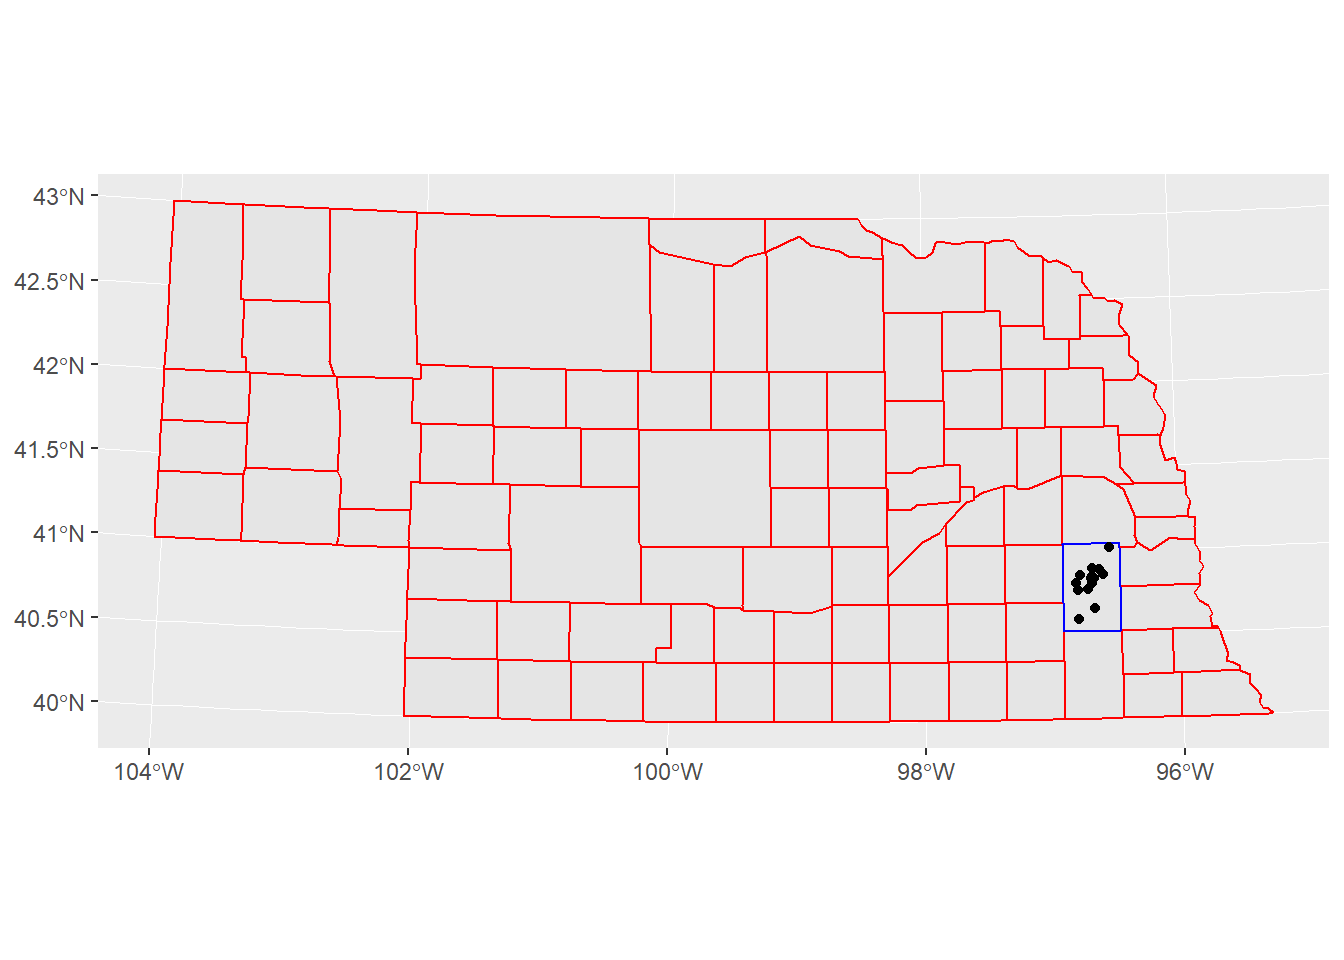
\includegraphics{A06_GLMs_files/figure-latex/unnamed-chunk-6-1.pdf}


\end{document}
